% Chapter Template

\chapter{Literature Review} % Main chapter title

\label{Chapter3} % Change X to a consecutive number; for referencing this chapter elsewhere, use \ref{ChapterX}

%----------------------------------------------------------------------------------------
%	SECTION 1
%----------------------------------------------------------------------------------------

\section{Introduction}
This section will go through the existing literature around the topic of GNSS spoofing and anti-spoofing. References were chosen based on their relevance in terms of
content as well as age. There have been some significant performance increases in technologies over the past 10 years.
This literature review will focus mainly on GNSS spoofing methods, with emphasis on the GPS constellation, and on potential anti-spoofing methods. While development of
anti-spoofing algorithms is not an aim of this thesis, knowledge of such methods allow for understanding potential attack vectors.

\section{Literature Review}
How GPS works has been covered in depth over the past few decades. The operating pricinpals for GPS and other GNSS systems is well known and was covered in the previous
chapter \ref{Chapter2}.

From literature the consensus is that the same thing that has made GPS ubiquitous with navigation and 
positioning has also made it a target for exploitation and manipulation. That is the workings
of the infrastructure are well known and public and are transparent and predictable \cite{RN7} \cite{RN4}. This is problematic since this infrastructure
is seen as a critical service by many industries including utility management, healthcare/ emergency services and security. \textcite{RN28} noted that the signals
presented to the receivers are usually trusted without any authentication or other checking. The authors show that this trust can be exploited without physical access to
or altering the software of the target device. One of the signal properties that makes spoofing simple is the received signal power from space which is less than -130dBm
making overpower the legitimate signal a simple task. Having such a system so prone to threats is not ideal. 

%
% Subsection - spoofing
%

\subsection{Spoofing Attack Literature} \label{Subsec:SpoofLit}
The further development of SDR platforms has driven down the cost of launching GNSS based spoofing attacks. Devices such as the Hack-RF, USRP, Blade-RF and others have
been documented for this use \cite{RN4} \cite{RN9}. These devices are all examples of Software defined radios that are capable of duplex operation. This combined with
open source software, as described in \cite{RN16} \cite{RN57} \cite{RN4}. The former is a software package, GPS-SDR, that converts a compatible SDR into a GPS receiver
wihtout any knowledge of GPS or signal procssing required. With some understanding this could be modified to capture the raw signal for use in a Meaconing spoofing
attack. The later refers to the setup and use of the GPS-SDR-SIM program. This program provides a method for producing a modulated GPS signal for transmission. It
requires the RINEX file for the date and time of the spoof attack as well as a set of coordinates to reproduce. Since it is open source it can be easily modified for any
use case. 

\textcite{RN28} created a spoofing device based on the HackRF SDR platform in conjunction with the open source program GPS-SIM-SDR. Hack-RF was chosen as the SDR platform
because of its open source nature, it also had the required specifications to perform the spoof attack. It was shown in this paper that the use of an SDR and open source
software was able to fool client devices such as apple smartphones into thinking they were else where. This included specific apps that require location data such as Uber
and DiDi. The authors provided a list of recommendations to minimise the risk of being spoofed. These recommendations are non trivial and some required alterations to how
the receiver processes the signal data.

\textcite{RN30} investigated the exact requirements for successfully spoofing a receiver. From the experiments it was found that there are 4 parameters that have required values in order to successfully spoof a GPS signal. That is the relative signal 
power must be $\geq+2dB$, the constant time offset must be $\leq 75ns$, location offset must be $\leq 500m$ and the relative time offset must be $\leq 80ns$. These values
correspond to situations where the reciver already has a lock on satellites. It was found that when values outside of those mentioned above, the lock would be lost and
the spoofing would be unsuccessful. The more victims that are trying to be spoofed the more restrictive the locaiton for performing the spoof becomes.

Software based GPS simulation tools similar to that of GPS-SDR-SIM have also been created using a combination of C and MATLAB \cite{RN15}. In this example the author used
C to ensure processing efficiency of the modulated signal, and used MATLAB to simulate multipath errors and uncertainty. The resultant file was then saved to the hard
drive of the host computer. This could then be loaded into an SDR for transmission, although this was not specifically touched on in the paper.

Over recent times there has been an increase in the industries that rely on the timing and postiional data provided by GNSS systems. One such industry is autonomous
vehicles, in particular drones. Drones can be used for hobbies, professional photography/ videography or for surveilance purposes. They are small and can be controlled from great
distances. All commercially available drones have some form of GNSS/GPS location service built in, and as such they become a target for spoofing attacks. Some drone
manufactueres have built in auto landing features in the event that the drone flys into restricted airspaces. This was to combat civilians who were flying within
airports, causing safety and security issues. This is one such way that spoofing attacks could be utelised now and in the future, by transmitting a signal that would make
the drone perceive itself to be in a restricted airspace and land. This kind of attack has been successfully conducted as shown in \cite{RN4}. 
\textcite{RN21} developed a system to perform a series of spoof attacks on UAV's based on an SDR \cite{RN23}. The goal of this was to be able to 
control the flight path of the UAV without raising any alarm's from the victim. This paper establishes the required conditions in which a UAV will
be susceptible to being captured from a spoofing attack, as well as the range of post capture control that the spoofer will have over the victim.
From testing it was found that spoof attacks were successful from up to 50m and up to a velocity of 10m/s.
Simulations were produced for analysis of post capture control of the UAV. 
When testing, both covert and overt spoofing methods were used, distinguished by whether or not the spoofer made an attempt to avoid detection. For the most part there
was no practical difference between covert and overt methods since the commercial GPS units did not trigger any anti spoof mechanism when being subjected to an overt
attack. Field testing showed that the spoof attempt caused unrecoverable navigation errors which resulted in the UAV crashing. Future work should increase the
sophistication of the attacks. This may decrease chances of the drone crashing due to unsuccessful attacks.

There has been research into ways that GPS spoofing attacks could be used in road navigation scenarios. \citeauthor{RN9} were able to implement an algorithm for road
network modelling and navigation spoofing using GPS. This algorithm coupled with a HackRF SDR meant that the authors were able to create a lunchbox sized spoofing device.
Although in research it was found that the victim devices were able to register a difference in location from network based sources and GNSS based sources, the victims
prioritised the location resolved from GNSS sources over network or cellular.
While this attack strategy may be successful against people not familiar with their surrounding area, someone who is familiar or is paying close attention should be able
to tell they are being led to an incorrect area. Where this is less likey to be the case is with driverless vechils.
In the paper written by \citeauthor{RN25} \cite{RN25} regarding driverless vehicle safety, it was noted that there is a significant threat to these types
of systems that rely heavily on reliable GPS signals. Although there have been proposed solutions to this problem through the use of 
other sensor information available locally to each vehicle and in the form of an ad-hoc network known as V2V (vehicle to vehicle) and more broadly
V2X (vehicle to everything) \cite{RN17}, this is still in its infancy and will require joint work from all vehicle manufacturers. 

\citeauthor{RN12} commented on the effect of GNSS spoofing of a cooperative victim. That is when someone is willing to aid the attacker
in performing an attack. This may be implemented to circumvent position based restrictions or if being GPS tracked during certain activities.
\citeauthor{RN12} used the example of a fisherman wanting their GNSS receiver to falsely report the boat had stayed out of protected areas \cite{RN12}.

In \citeyear{RN6} \textcite{RN6} investigated the different spoofing and antispoofing techniques available. \citeauthor{RN6} noted that spoofing attacks can be divided into 3 main categories:
GPS signal simulator, Receiver-Based spoofers and Sophisticated Receiver based spoofers. These attack strategies come about because of vulnerabilities in the GPS system.
These vulnerabilities can be described in the three operational layers of GPS, signal processing, data bit, and position/navigation solutions.
Testing spoofing techniques is difficult to achieve since there are regulations around the emission of EM radiation at certain frequencies and power levels.
There were three methods used to test the spoofing/antispoofing techniques. These were Indoor re-transmissions, spoofing using recorded data (No RF transmission), and
using RF combiners to combine authentication and spoofed signals.
The results that were acquired showed that the commercial GPS receivers were vulnerable to a number of spoofing techniques.
Previous research into the effects of spoofing can be found in \cite{RN23}. This predates more modern methods for launching a successful spoofing attack and uses a
specialised DSP chip within a specilised hardware configuration. The findings of this paper was used to recommend anti-spoofing methods for unsophisticated spoofing
attacks. \citeauthor{RN23} was able to implement complex spoofing setups with multiple phase locked radios that were able to overcome some anti-spoofing techniques. 

\begin{figure}[h]
    \begin{centering}
        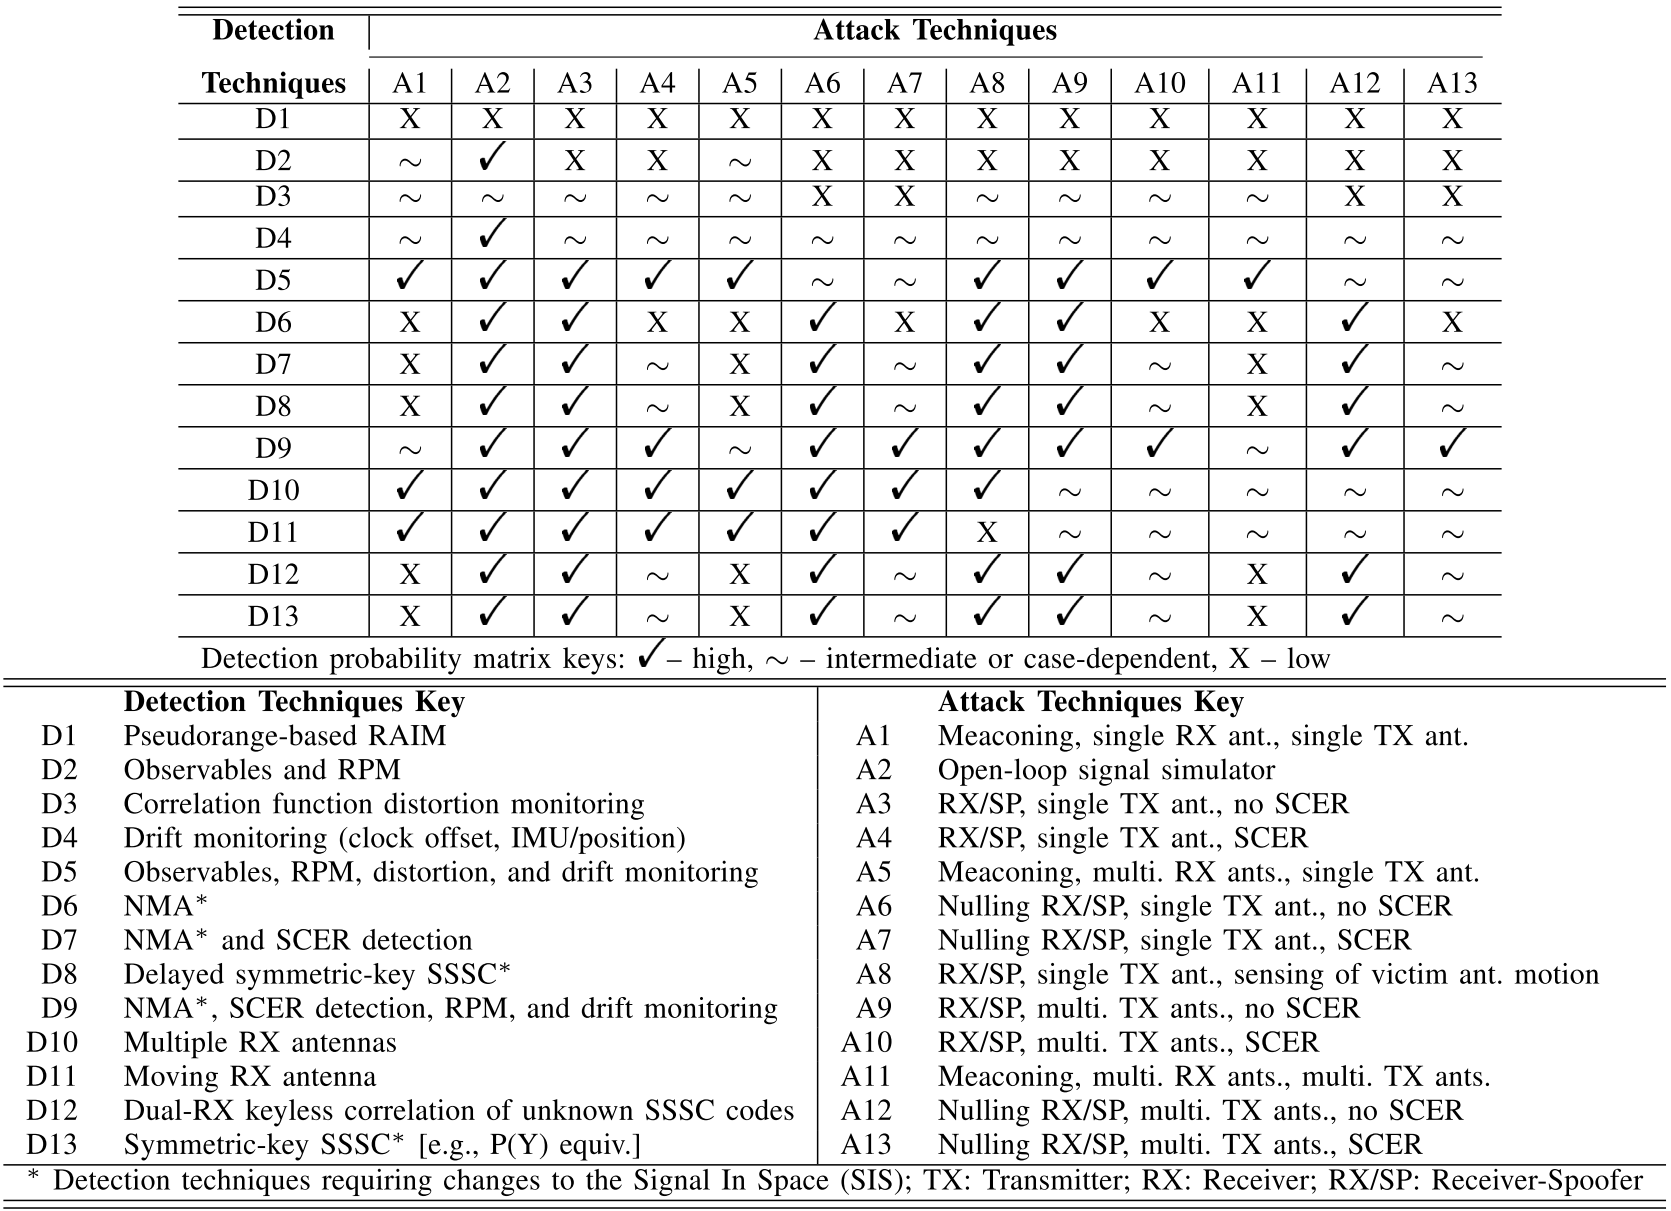
\includegraphics[width=14cm, keepaspectratio]{Figures/Attack and defence summary.png}
        \caption{Summary of spoofing attack and defence methods and their effectiveness against each other as found in \cite{RN12}}
    \label{fig:SpoofDefenceSumm}
    \end{centering}
\end{figure}

%
% Subsection - Anti-spoofing
%

\subsection{Anti-Spoofing Literature}
It is common within research to investigate methods of spoofing attack and to combine this with recommendations for anti-spoofing. This was the case with \textcite{RN6}
and \textcite{RN23}. The later, as mentioned above in Section \ref{Subsec:SpoofLit} a spoofing device was developed and tested against some anti-spoofing methods. From
this anti-spoofing recommendations were developed. The recommedations are as per \citeauthor{RN6}.
\textcite{RN6} investigated antispoofing techniques available. Antispoofing can be broken down into 2 groups spoof detection and spoof mitigation, with each of these being able to be further broken into subcategories.
The effectiveness of each spoof detection technique was tabulated and compared. As was the spoof mitigation techniques. Each detection and mitigation
method was given a complexity, effectiveness and spoofing scenario generality rating with notes made about the received capability requirements and are summarised in
Table \ref{tab:SpoofDetectSum} and Table \ref{tab:SpoofMitigateSum}. It was 
shown that with modest, low complexity spoof detection and mitigation strategies some of the spoof attacks were able to be overcome.

\renewcommand{\arraystretch}{1.2}
\begin{table}[ht]
    \begin{center}
        \caption{Summary of Spoofing Detection Methods from \cite{RN6}}
        \label{tab:SpoofDetectSum}
        \makebox[1 \textwidth][c]{
        \resizebox{1.1 \textwidth}{!} {
            \begin{tabular}{ m{40mm}|m{35mm}|c|c|m{30mm}|m{20mm} }
                \hline
                \textbf{Anti-Spoofing method} & \textbf{Spoofing Feature} & \textbf{Complexity} & \textbf{Effectiveness} &
                \textbf{Receiver required capability} & \textbf{Spoofing scenario generality} \\
                \hline
                $C/N_0$ monitoring & Higher $C/N_0$ & Low & Medium & $C/N_0$ monitoring & Medium \\
                Absolute power monitoring & Higher amplitude & Low & Medium & Absolute power monitoring & High \\
                Power variation versus receiver movement & Higher power variations due to proximity & Low & Low & Antenna movement/ $C/N_0$ monitoring & Low \\
                L1/L2 power comparison & No L2 signal for spoofer & Medium & Low & L2 reception capability & Low \\
                Direction of arrival comparison & Spoofing signals coming from the same direction & High & High & Multiple receiver antennas & High \\              
                Pairwise correlation in synthetic array & Spoofing signals coming from the same direction & Low & High & Measuring correlation coefficient & High \\
                TOA discrimination & Inevitable delay of spoofing signal & Medium & Medium & TOA analysis & Low \\
                Signal quality monitoring & Deviated shape of authentic correlation peak & Medium & Medium & Multiple correlators & Low \\
                Distribution analysis of the correlator output & Perturbed amplitude distribution due to spoofing-authenntic interaction & Low & Medium & Distribution
                analysis of correlator outputs & Medium \\
                Consistency check with other solutions & Inconsistency of spoofing solution & High & High & Different navigation sensors & High \\
                Cryptographic authentication & Not authenticated & High & High & Authentication & High \\
                Code and phase rate consistency check & Mismatch between artifical code and phase rate & Low & Low & - & Low \\
                GPS clock consistency check & Spoofing/authentic clock inconsistency & Low & Medium & - & Medium \\ 
                \hline
            \end{tabular}
        }
        }
    \end{center}
\end{table}
\renewcommand{\arraystretch}{1}

\renewcommand{\arraystretch}{1.2}
\begin{table}[ht]
    \begin{center}
        \caption{Summary of Spoofing Mitigation Methods from \cite{RN6}}
        \label{tab:SpoofMitigateSum}
        \makebox[1 \textwidth][c]{
        \resizebox{1.1 \textwidth}{!} {
            \begin{tabular}{ m{40mm}|m{35mm}|c|c|m{30mm}|m{20mm} }
                \hline
                \textbf{Anti-Spoofing method} & \textbf{Spoofing Feature} & \textbf{Complexity} & \textbf{Effectiveness} &
                \textbf{Receiver required capability} & \textbf{Spoofing scenario generality} \\
                \hline
                Vestigial signal detection & The authentic signal is still present and can be detected & High & Medium & Multiple receive channels & Medium \\ 
                Multi-antenna null steering & Spoofing signals coming from same direction & Medium & High & Multiple receive antennas & High \\
                RAIM & Higher residuals for spoofed measurements & Medium & Medium & - & Medium \\
                \hline
            \end{tabular}
            }
            }
    \end{center}
\end{table}
\renewcommand{\arraystretch}{1}

\section{Literature Review Conclusion}
Some of the early assessments of the spoofing threat included methods for performing said attacks using specialised hardware \cite{RN23}. This increased the technical
knowledge required to be able to perform an attack.
